\documentclass[xcolor={usenames,dvipsnames,svgnames,table}]{beamer}

\mode<presentation>
\usetheme{Madrid}

\usecolortheme[RGB={80,0,0}]{structure}
\useoutertheme[subsection=false]{miniframes}
\useinnertheme{default}

% hide navigation controlls
\setbeamertemplate{navigation symbols}{}

\setbeamercolor{normal text}{fg=black}
\setbeamercovered{dynamic}
\beamertemplatetransparentcovereddynamicmedium
\setbeamertemplate{caption}[numbered]

\definecolor{Maroon}{RGB}{80,0,0}
\definecolor{BurntOrange}{RGB}{204,85,0}

% load macros and prevent authblk from loading
\makeatletter
% prevent a package from loading
\newcommand{\dontusepackage}[2][]{%
    \@namedef{ver@#2.sty}{9999/12/31}%
    \@namedef{opt@#2.sty}{#1}
}

% a macro to load packages only if they are not yet loaded, needed for combination of beamer and hyperref
\newcommand{\usepackagesave}[2][{}]{
    \ltx@ifpackageloaded{#2}{}{
        \usepackage[#1]{#2}}
}
\makeatother
\dontusepackage{authblk}

% load packages, settings and definitions
% this file contains all commonly used packages for the Rattlesnake documentation
% new package, add comment what they are used for

% command packages
\usepackage{xifthen}     % if -then else command

% language and font improvements
\usepackage[english]{babel}	% Multilingual support - https://www.ctan.org/pkg/babel
\usepackage[utf8]{inputenc} % Accept different input encodings - https://www.ctan.org/pkg/inputenc
\usepackage[kerning,spacing,babel]{microtype} % Subliminal refinements towards typographical perfection - https://www.ctan.org/pkg/microtype
\usepackage{eepic}      % Extensions to epic - https://www.ctan.org/pkg/eepic
\usepackage{epic}       % Enhance LaTeX picture mode - https://www.ctan.org/pkg/epic
\usepackage[T1]{fontenc} % selecting font encodingsselecting font encodings - https://www.ctan.org/pkg/fontenc
\usepackage{lmodern}

% title packages
\usepackage{authblk}		% footnote style author/affiliation - https://www.ctan.org/pkg/authblk

% symbols
\usepackage{upgreek}		% Upright Greek letters - https://www.ctan.org/pkg/upgreek
\usepackage{cancel}			% \cancel cmd - https://www.ctan.org/pkg/cancel

% chemical and isotope packages
\usepackage{isotope}		% isotope command - https://www.ctan.org/pkg/isotope
\usepackage{mhchem}			% chemical formulae/equations - https://www.ctan.org/pkg/mhchem

% layout packages
\usepackage{xspace}			% smart space \xspace - https://www.ctan.org/pkg/xspace
\usepackage{icomma}			% smart math comma - https://www.ctan.org/pkg/icomma
\usepackage{chngpage}		% page layout change during document - https://www.ctan.org/pkg/chngpage
\usepackage[usenames,dvipsnames,svgnames,table]{xcolor}			% color definitions - https://www.ctan.org/pkg/xcolor
\usepackage{enumitem}   % layout for itemize and enumerate - http://www.ctan.org/pkg/enumitem
\usepackage{setspace}    % allows for \singlespacing, \onehalfspacing, and \doublespacing commands - https://www.ctan.org/pkg/setspace

% floating packages
% needed by the breakalgo environment labelsep=quad
\usepackage[singlelinecheck=false, labelsep=quad]{caption}	% table captions - https://www.ctan.org/pkg/caption
\usepackage{subcaption}		% Support for sub-captions - https://www.ctan.org/pkg/subcaption
\usepackage{placeins}   	% Control float placement - https://www.ctan.org/pkg/placeins
\usepackage{float}      	% Improved interface for floating objects - https://www.ctan.org/pkg/float

% table packages
\usepackage{supertabular}	% multi-page tables package - https://www.ctan.org/pkg/supertabular
\usepackage{booktabs}		% table settings - https://www.ctan.org/pkg/booktabs
\usepackage{array}			% Extending the array and tabular environments - https://www.ctan.org/pkg/array
\usepackage{multirow}		% tabular cells spanning multiple rows - https://www.ctan.org/pkg/multirow
% \usepackage{tabls}      % Better vertical spacing in tables and arrays - https://www.ctan.org/pkg/tabls
\usepackage{colortbl}      % Allows for color manipulation within tables - https://www.ctan.org/pkg/colortbl
\usepackage{makecell}

% pictures, plots and listings
\usepackage{graphicx}		% include graphics - https://www.ctan.org/pkg/graphicx
\usepackage{wrapfig}		% wrapfigure enviroment - https://www.ctan.org/pkg/wrapfig
\usepackage{pgfplots}		% latex plots - https://www.ctan.org/pkg/pgfplots
%\usepackage{subfigure}


% source code and algorithms
\usepackage{algorithmicx} % newer version of algorithmic - https://www.ctan.org/pkg/algorithmicx
\usepackage{listings} 	% source code listings - http://www.ctan.org/pkg/listings
\usepackage{verbatim}   % verbatim - https://www.ctan.org/pkg/verbatim

% misc packages
\usepackage{url}        % provide \url command for web addresses - https://www.ctan.org/pkg/url
\usepackage{import}			% Establish input relative to a directory - https://www.ctan.org/pkg/import
\usepackage{afterpage}  % Execute command after the next page break - https://www.ctan.org/pkg/afterpage
\usepackage{lscape}     % Place selected parts of a document in landscape - https://www.ctan.org/pkg/lscape
\usepackage{rotating}   % Rotation tools, including rotated full-page floats - https://www.ctan.org/pkg/rotating
\usepackage{chngcntr}   % Change the resetting of counters - http://ctan.org/pkg/chngcntr
\usepackage{textpos}    % Allows logo and banner manipulation

% eps support
\usepackage{epsfig}       % include eps figures - https://www.ctan.org/pkg/epsfig
\usepackage{epsf}          % Simple macros for EPS inclusion - https://www.ctan.org/pkg/epsf
\usepackage{epstopdf}   %use .eps images (as pdf) in \includegraphics


% reference packages
% hyperref must be loaded before amsmath to avoid problems with subequations and align
\usepackage{hyperref}		% Extensive support for hypertext - https://www.ctan.org/pkg/hyperref


% packages that must be loaded after hyperref - http://tex.stackexchange.com/questions/1863/which-packages-should-be-loaded-after-hyperref-instead-of-before
\usepackage{geometry}		% Flexible and complete interface to document dimensions - https://www.ctan.org/pkg/geometry
\usepackage{algorithm}  % algorithm enviroment

% ams math packages
\usepackage{amsmath}    % mathematical facilities - https://www.ctan.org/pkg/amsmath
\usepackage{amsfonts}   % fonts for math - https://www.ctan.org/pkg/amsfonts
\usepackage{amssymb}    %
\usepackage{amsthm}     % Typesetting theorems - https://www.ctan.org/pkg/amsthm

\usepackage{nameref}		% allows references with names instread of numbers \nameref - http://www.ctan.org/pkg/nameref
\usepackage[capitalize,nameinlink]{cleveref}   % smart references - http://ctan.org/pkg/cleveref
\usepackage{tikz}
\usepackage{grffile}

% general settings
\renewcommand\floatpagefraction{0.75} % threshold for floating objects to be placed on a page

\makeatletter
% center floats generally
\g@addto@macro\@floatboxreset\centering
% gives the current section name
\newcommand*{\currentname}{\@currentlabelname}
\makeatother

% figure setting, controlles the height of pgfplots from the main script
\newlength{\figheight}
\setlength{\figheight}{12cm}

% example for hyperref setup, we have to see if we can get that better
\hypersetup{
  linktocpage=true,       % links in table of contents
  bookmarks=true,         % show bookmarks bar?
  unicode=true,           % non-Latin characters in Acrobat's bookmarks
  pdftoolbar=true,        % show Acrobat's toolbar?
  pdfmenubar=true,        % show Acrobat's menu?
  pdffitwindow=false,     % window fit to page when opened
  pdfstartview={FitH},    % fits the width of the page to the window
  pdfnewwindow=true,      % links in new window
  colorlinks=false,       % false: boxed links; true: colored links
  linkcolor=red,          % color of internal links
  citecolor=green,        % color of links to bibliography
  filecolor=magenta,      % color of file links
  urlcolor=cyan,          % color of external links
  pdfborder={0 0 0},      % color of link frames
}


% set package versions
\pgfplotsset{compat=1.12}

% set table and figure counters here

% set up listings - see https://en.wikibooks.org/wiki/LaTeX/Source_Code_Listings
\lstset{ %
  backgroundcolor=\color{white},   % choose the background color; you must add \usepackage{color} or \usepackage{xcolor}; should come as last argument
  basicstyle=\footnotesize,        % the size of the fonts that are used for the code
  breakatwhitespace=false,         % sets if automatic breaks should only happen at whitespace
  breaklines=true,                 % sets automatic line breaking
  captionpos=b,                    % sets the caption-position to bottom
  commentstyle=\color{Gray},       % comment style
  deletekeywords={...},            % if you want to delete keywords from the given language
  escapeinside={\%*}{*)},          % if you want to add LaTeX within your code
  extendedchars=true,              % lets you use non-ASCII characters; for 8-bits encodings only, does not work with UTF-8
  frame=single,	                   % adds a frame around the code
  keepspaces=true,                 % keeps spaces in text, useful for keeping indentation of code (possibly needs columns=flexible)
  keywordstyle=\color{blue},       % keyword style
  morekeywords={*,...},            % if you want to add more keywords to the set
  numbers=left,                    % where to put the line-numbers; possible values are (none, left, right)
  numbersep=5pt,                   % how far the line-numbers are from the code
  numberstyle=\tiny\color{Gray},   % the style that is used for the line-numbers
  rulecolor=\color{black},         % if not set, the frame-color may be changed on line-breaks within not-black text (e.g. comments (green here))
  showspaces=false,                % show spaces everywhere adding particular underscores; it overrides 'showstringspaces'
  showstringspaces=false,          % underline spaces within strings only
  showtabs=false,                  % show tabs within strings adding particular underscores
  stepnumber=2,                    % the step between two line-numbers. If it's 1, each line will be numbered
  stringstyle=\color{mymauve},     % string literal style
  tabsize=2,	                     % sets default tabsize to 2 spaces
  title=\lstname                   % show the filename of files included with \lstinputlisting; also try caption instead of title
}

% define style for moose
\lstdefinestyle{cpp}{
  belowcaptionskip=1\baselineskip,
  breaklines=true,
  frame=TB,
  xleftmargin=\parindent,
  language=C,
  showstringspaces=false,
  basicstyle=\footnotesize\ttfamily,
  keywordstyle=\bfseries\color{green!40!black},
  commentstyle=\itshape\color{purple!40!black},
  identifierstyle=\color{blue},
  stringstyle=\color{orange},
}

\lstdefinestyle{python}{
  belowcaptionskip=1\baselineskip,
  breaklines=true,
  frame=,
  xleftmargin=\parindent,
  language=Python,
  showstringspaces=false,
  basicstyle=\footnotesize\ttfamily,
  keywordstyle=\bfseries\color{blue},
  commentstyle=\itshape\color{gray},
  identifierstyle=\color{black},
  stringstyle=\color{green},
}

\lstdefinelanguage{Moose}{
  morekeywords={one,two,three,four,five,six,seven,eight,
  nine,ten,eleven,twelve,o,clock,rock,around,the,tonight},
  sensitive=false,
  morecomment=[l]{//},
  morecomment=[s]{/*}{*/},
  morestring=[b]",
}

\lstdefinestyle{moose}{
  belowcaptionskip=1\baselineskip,
  breaklines=true,
  frame=tb,
  xleftmargin=\parindent,
  language=Moose,
  showstringspaces=false,
  basicstyle=\footnotesize\ttfamily,
  keywordstyle=\bfseries\color{blue},
  commentstyle=\itshape\color{gray},
  identifierstyle=\color{black},
  stringstyle=\color{green},
}

\lstset{literate=
  {á}{{\'a}}1 {é}{{\'e}}1 {í}{{\'i}}1 {ó}{{\'o}}1 {ú}{{\'u}}1
  {Á}{{\'A}}1 {É}{{\'E}}1 {Í}{{\'I}}1 {Ó}{{\'O}}1 {Ú}{{\'U}}1
  {à}{{\`a}}1 {è}{{\`e}}1 {ì}{{\`i}}1 {ò}{{\`o}}1 {ù}{{\`u}}1
  {À}{{\`A}}1 {È}{{\'E}}1 {Ì}{{\`I}}1 {Ò}{{\`O}}1 {Ù}{{\`U}}1
  {ä}{{\"a}}1 {ë}{{\"e}}1 {ï}{{\"i}}1 {ö}{{\"o}}1 {ü}{{\"u}}1
  {Ä}{{\"A}}1 {Ë}{{\"E}}1 {Ï}{{\"I}}1 {Ö}{{\"O}}1 {Ü}{{\"U}}1
  {â}{{\^a}}1 {ê}{{\^e}}1 {î}{{\^i}}1 {ô}{{\^o}}1 {û}{{\^u}}1
  {Â}{{\^A}}1 {Ê}{{\^E}}1 {Î}{{\^I}}1 {Ô}{{\^O}}1 {Û}{{\^U}}1
  {œ}{{\oe}}1 {Œ}{{\OE}}1 {æ}{{\ae}}1 {Æ}{{\AE}}1 {ß}{{\ss}}1
  {ű}{{\H{u}}}1 {Ű}{{\H{U}}}1 {ő}{{\H{o}}}1 {Ő}{{\H{O}}}1
  {ç}{{\c c}}1 {Ç}{{\c C}}1 {ø}{{\o}}1 {å}{{\r a}}1 {Å}{{\r A}}1
  {€}{{\euro}}1 {£}{{\pounds}}1
}

% Common style and macro defintions for CLASS documents
%=================================================================================================

%%% General Commands

%% structural elements
% An explanation for a function
\newcommand{\explain}[1]{\mbox{\hspace{2em} #1}}
% attemtion box
\newcommand{\attention}[1]{\mbox{\hspace{2em} #1}}
% comments at the sde of the paragraph
\newcommand{\sidenotes}[1]{\marginpar{ {\footnotesize #1} }}
% create empty double page, TODO do we need that?
\newcommand{\clearemptydoublepage}{\newpage{\pagestyle{empty}\cleardoublepage}}
%TODO description here
\newcommand{\apost}{\textit{a posteriori\xspace}}
%TODO description here
\newcommand{\Apost}{\textit{A posteriori}\xspace}

%%% Math
%% Paratnhis etc.
% ()
\newcommand{\parenthesis}[1]{{\left(#1 \right)}}
% []
\newcommand{\bracket}[1]{{\left[ #1 \right]}}
% {}
\newcommand{\bracet}[1]{{\left\{#1 \right\}}}
% <>
\newcommand{\angled}[1]{{\left\langle#1\right\rangle}}

%% common math symbols
% imaginary number
\newcommand{\img}{\ensuremath{\hat{\imath}}\xspace}
% gradient symbol
\newcommand{\grad}{\vec{\nabla}}
\newcommand{\del}{\vec{\nabla}}
% adjoint
\newcommand{\adj}[2][{}]{{{#2}^{\dagger#1}}}
% order number
\newcommand{\order}[1]{^\parenthesis{#1}}
% iteration number
\newcommand{\iter}[1]{^{#1}}

%% common math function
% divergence
\renewcommand{\div}{\del\! \cdot \!}
% rotation
\newcommand{\rot}{\del\! \times \!}
% absolute value
\newcommand{\abs}[1]{\left|#1\right|}
% norm
\newcommand{\norm}[2][{}]{\lVert#2\rVert_{#1}}
% e function
\newcommand{\e}[1]{\mathrm{e}^{#1}}
% power of ten
\newcommand{\tento}[1]{\ensuremath{10^{#1}}\xspace}
% E notation
\newcommand{\E}[1]{\ensuremath{\cdot \tento{#1}}\xspace}
% sign
\DeclareMathOperator{\sign}{sign}

%% fraction
% 1 / 2
\newcommand{\half}[1][1]{\frac{#1}{2}}
% 1 / 3
\newcommand{\third}[1][1]{\frac{#1}{3}}
% 1 / 4
\newcommand{\fourth}[1][1]{\frac{#1}{4}}

% vectors etc
% vector, we use standard latex notation
% matrix
\newcommand{\mat}[1]{\mathbf{#1}}
% tensor
\newcommand{\tensor}[1]{\underline{\underline{#1}}}
% operator symbol
\newcommand{\op}[1]{\mathrm{\mathbf{#1}}}

% derivatives
% first derivatives
% general first derivative, with optional argument for f
\newcommand{\dd}[2][]{\frac{\partial #1}{\partial #2}}
% partial derivative for x, optional argument for f
\newcommand{\ddx}[1][]{\dd[#1]{x}}
% partial derivative for y, optional argument for f
\newcommand{\ddy}[1][]{\dd[#1]{y}}
% partial derivative for z, optional argument for f
\newcommand{\ddz}[1][]{\dd[#1]{z}}
% partial derivative for t, optional argument for f
\newcommand{\ddt}[1][]{\dd[#1]{t}}

% second derivatives, only for a single variable, cross derivatives are too many
% second general derivative, optional argument for f
\newcommand{\ddd}[2][{}]{\frac{\partial^2 #1}{\partial {#2}^2}}
% second partial derivative for x, optional argument for f
\newcommand{\ddxx}[1][]{\ddd[#1]{x}}
% second partial derivative for y, optional argument for f
\newcommand{\ddyy}[1][]{\ddd[#1]{y}}
% second partial derivative for z, optional argument for f
\newcommand{\ddzz}[1][]{\ddd[#1]{z}}
% second partial derivative for t, optional argument for f
\newcommand{\ddtt}[1][]{\ddd[#1]{t}}

% integrals
% integral dx, optional parameter for different variable
\newcommand{\dx}[1][x]{\,d#1}
% integral dy
\newcommand{\dy}{\dx[y]}
% integral dz
\newcommand{\dz}{\dx[z]}
% integral dt
\newcommand{\dt}{\dx[t]}
%integral dmu
\newcommand{\dmu}{\dx[\mu]}
%integral dOmega
\newcommand{\domg}{\dx[\direction]}

% spherical integrals
% shortcut for sphere notation
\newcommand{\sphere}{\ensuremath{\mathcal{S}}\xspace}
% angular quadrature weight
\newcommand{\aqweight}{\omega}

% integral over full sphere
\newcommand{\intsp}{\int_{4\pi}}
% integral over half sphere
\newcommand{\inthalfsp}{\int_{2\pi}}
% polar integral
\newcommand{\intpolar}{\int_{-1}^{1}}
% negative partial polar integral
\newcommand{\intnpolar}{\int_{-1}^{0}}
% positive partial polar integral
\newcommand{\intppolar}{\int_{0}^{1}}


% FEM symbols
% spatial domain
\newcommand*{\domain}{\ensuremath{\mathcal{D}}\xspace}
% boundary of a spatical domain
\newcommand*{\boundary}{\ensuremath{{\partial\domain}}\xspace}
% vacuum boundary of a spatical domain
\newcommand*{\vboundary}{\ensuremath{{\boundary}_v}\xspace}
% reflective boundary of a spatical domain
\newcommand*{\rboundary}{\ensuremath{{\boundary}_r}\xspace}
% interface surface
\newcommand*{\interface}{\ensuremath{{\Gamma}}\xspace}
% general and isotropic test function
\newcommand{\testfct}{\ensuremath{\phi^{*}}\xspace}
% angular test function
\newcommand{\atestfct}{\ensuremath{\psi^{*}}\xspace}
% surface normal
\newcommand{\normal}{\ensuremath{\vec{n}}\xspace}
% boundary normal
\newcommand{\bnormal}{\ensuremath{\normal_\mathrm{b}}\xspace}

% DFEM commands
% interface jump
\newcommand{\jump}[1]{[\![#1]\!]}
% what is the different?
\newcommand{\jmpa}[1]{[\![\![#1]\!]\!]}
% mean value
\newcommand{\meanval}[1]{\{\!\!\{#1\}\!\!\}}

% common physical symbols
% mass stream
\newcommand{\mdot}{\ensuremath{\dot{m}}\xspace}

% nuclear symbols
% Sn
\newcommand{\sn}[1][N]{\ensuremath{S_#1}\xspace}
% Pn
\newcommand{\pn}[1][N]{\ensuremath{P_#1}\xspace}
% keff
\newcommand{\keff}{\ensuremath{k_{\text{eff}}}\xspace}
% kinf
\newcommand{\kinf}{\ensuremath{k_{\text{inf}}}\xspace}

% transport symbols
\newcommand{\addgroup}[1]{\ifthenelse{\isempty{#1}}{}{_{#1}}}
% direction omega
\newcommand{\direction}{\ensuremath{\vec{\Omega}}\xspace}
% direction omega
\newcommand{\position}{\ensuremath{\vec{x}}\xspace}
% current
\newcommand{\current}[1][]{\ensuremath{\vec{J}\addgroup{#1}}\xspace}
% positive half range current
\newcommand{\ppcurrent}[1][]{\ensuremath{\hat{\jmath}\,^+\addgroup{#1}}\xspace}
% negative half range current
\newcommand{\npcurrent}[1][]{\ensuremath{\hat{\jmath}\,^-\addgroup{#1}}\xspace}
% drift vector
\newcommand{\drift}[1][]{\ensuremath{\hat{D}\addgroup{#1}}\xspace}
% local diffusion coefficient
\newcommand{\DC}[1][]{\ensuremath{\mathrm{D}\addgroup{#1}}\xspace}
% nonlocal diffusion tensor
\newcommand{\DCNL}[1][]{\ensuremath{\tensor{\mathrm{D}}\addgroup{#1}}\xspace}
% cross section label
\newcommand{\xslabel}[2][]{\ifthenelse{\isempty{#1}}{\mathrm{#2}}{\mathrm{#2},#1}}
% total cross section
\newcommand{\sigt}[1][]{\ensuremath{\sigma_{\xslabel[#1]{t}}}\xspace}
% scattering cross section
\newcommand{\sigs}[1][]{\ensuremath{\sigma_{\xslabel[#1]{s}}}\xspace}
% fission cross section
\newcommand{\sigf}[1][]{\ensuremath{\sigma_{\xslabel[#1]{f}}}\xspace}
% removal cross section
\newcommand{\sigr}[1][]{\ensuremath{\sigma_{\xslabel[#1]{r}}}\xspace}
% absorption cross section
\newcommand{\siga}[1][]{\ensuremath{\sigma_{\xslabel[#1]{a}}}\xspace}
% transport cross section
\newcommand{\sigtr}[1][]{\ensuremath{\sigma_{\xslabel[#1]{tr}}}\xspace}
% scattering moment
\newcommand{\sigl}[2][{}]{\ensuremath{\sigma_{#2#1}}\xspace}

% total cross section
\newcommand{\Sigt}[1][]{\ensuremath{\Sigma_{\xslabel[#1]{t}}}\xspace}
% scattering cross section
\newcommand{\Sigs}[1][]{\ensuremath{\Sigma_{\xslabel[#1]{s}}}\xspace}
% fission cross section
\newcommand{\Sigf}[1][]{\ensuremath{\Sigma_{\xslabel[#1]{f}}}\xspace}
% removal cross section
\newcommand{\Sigr}[1][]{\ensuremath{\Sigma_{\xslabel[#1]{r}}}\xspace}
% absorption cross section
\newcommand{\Siga}[1][]{\ensuremath{\Sigma_{\xslabel[#1]{a}}}\xspace}
% transport cross section
\newcommand{\Sigtr}[1][]{\ensuremath{\Sigma_{\xslabel[#1]{tr}}}\xspace}
% scattering moment
\newcommand{\Sigl}[2][{}]{\ensuremath{\Sigma_{#2#1}}\xspace}

% spatial weight function
\newcommand{\weight}[1][]{\ensuremath{w\addgroup{#1}}\xspace}

% physical units
% general style for a unit symbol
\newcommand{\unit}[1]{\mathrm{#1}}
% distance
% meter maybe \meter better and more clear?
\newcommand{\m}{\,\unit{m}\xspace}
% centimeter
\newcommand{\cm}{\,\unit{cm}\xspace}
% milimeter
\newcommand{\mm}{\,\unit{mm}\xspace}

% time
% second
\newcommand{\s}{\,\unit{s}\xspace}

% transport units
% scalar flux
\newcommand{\sfluxunit}{\,\ensuremath{\frac{1}{\unit{cm}^2\unit{s}}}\xspace}
% angular flux
\newcommand{\afluxunit}{\,\ensuremath{\frac{1}{\unit{cm}^2\unit{s}\cdot\unit{st}}}\xspace}
% diffusion coefficient
\newcommand{\dcunit}{\,\ensuremath{\unit{cm}}\xspace}


% \newenvironment{myverbatim}%            To change the pseudocode font
% {\par\noindent%
%  \rule[0pt]{\linewidth}{0.2pt}
%  \vspace*{-9pt}
%  \linespread{0.0}\small\verbatim}%
% {\rule[-5pt]{\linewidth}{0.2pt}\endverbatim}
%
% \newenvironment{myverbatim1}%            To change the pseudocode font
% {\par\noindent%
%  \rule[0pt]{\linewidth}{0.2pt}
%  \vspace*{-9pt}
%  \linespread{1.0}\scriptsize\verbatim}%
% {\rule[-5pt]{\linewidth}{0.2pt}\endverbatim}


% nicer item settings
\setlist[1]{nolistsep,label=\(\textcolor{Maroon}{\blacksquare}\)}
\setlist[2]{nolistsep,label=\(\textcolor{Maroon}{\bullet}\)}

\setenumerate[1]{
	label=\protect\usebeamerfont{enumerate item}%
	\protect\usebeamercolor[fg]{enumerate item}%
	\insertenumlabel.
}

%%%%%%%%%%%%%%%%%%%%%%%%%%%%%%%%%%%%%%%%%%%%%%%
%%% edit to fit your document

% set up pdf support and indexing
\hypersetup{
    pdftitle={<Title>},
    pdfauthor={<author>},
    pdfsubject={<subject>},
    pdfkeywords={<keywords>},
}

\title[Final Project]{Final Project: Attack Detection}
\author[Hardy, Behne, German, Vijaykumar \& Singh]{
	Zachary Hardy (Team Captain), Patrick Behne, Peter German, \\ Akhilesh Vijaykumar, Harpreet Singh
}
\institute[Texas A\&M]{CSCE 633 \\ Texas A\&M University}
\date[April 27, 2020]{April 27, 2020}

\begin{document}

% title page, do not edit
{
\setbeamertemplate{headline}[default] 
\begin{frame}
\vfill
\titlepage
\vfill
%\begin{figure}[t]
%	\centering
%	\includegraphics[width=.5\textwidth]{images/nuen}
%\end{figure}
%\vfill
\end{frame}
}

%%%%%%%%%%%%%%%%%%%%%%%%%%%%%%%%%%%%%%%%%%%%%%%%%%%%%%%%%%%%%%%%%%%%%%%%%%%%%%%%%%%%%%%%%%%%%%%%%%%%%%%%%%%
\section{Introduction}	% define sections here, it is possible to get section slides automatically, but this is not enabled
\subsection{}	% we have to keep these to get the navigation
%%%%%%%%%%%%%%%%%%%%%%%%%%%%%%%%%%%%%%%%%%%%%%%%%%%%%%%%%%%%%%%%%%%%%%%%%%%%%%%%%%%%%%%%%%%%%%%%%%%%%%%%%%%

\begin{frame}[t]\frametitle{Outline}
\tableofcontents
 \end{frame}
 
%%%%%%%%%%%%%%%%%%%%%%%%%%%%%%%%%%%%%%%%%%%%%%%%%%%%%%%%%%%%%%%%%%%%%%%%%%%%%%%%%%%%%%%%%%%%%%%%%%%%%%%%%%%%%%

\section{Input Transformations}
\subsection{}

\begin{frame}[t]\frametitle{Input Transformations}
	\begin{itemize}
		\item Transformations only on training data to remove bias. \vspace*{0.05in}
		
		\item Normalization across all samples or samples sharing a time-stamp. \vspace*{0.05in}
		
		\item Available feature-wise normalization techniques:
		\begin{itemize}
			
			\item Max: Map $X$ to $X \in \left[ \frac{X_{\min}}{X_{\max}}, 1\right]$. \\
			
			\item Standard: Map $X$ to a zero mean and unit variance. \\
			
			\item Robust: Map $X$ by removing the median and dividing with the IQR. \\
			
		\end{itemize} \vspace*{0.05in}
		
		\item Principal Component Analysis (PCA):
		\begin{itemize}
			\item Dimensionality reduction.
			\item Fully decouple the inputs by changing to an orthogonal coordinate system.
		\end{itemize}	
	\end{itemize}
\end{frame}

\begin{frame}[t]\frametitle{Singular Value Decomposition of Input Data}
	\begin{figure}[H]
		\centering
		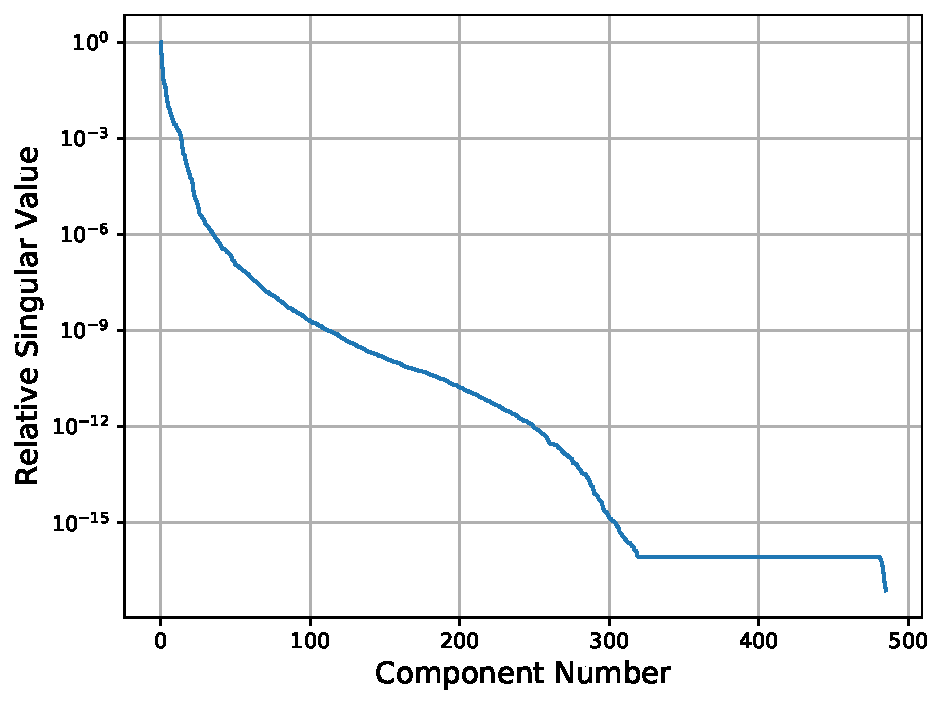
\includegraphics[scale=0.5]{../report/figures/pca.pdf}
	\end{figure}
\end{frame}


%%%%%%%%%%%%%%%%%%%%%%%%%%%%%%%%%%%%%%%%%%%%%%%%%%%%%%%%%%%%%%%%%%%%%%%%%%%%%%%%%%%%%%%%%%%%%%%%%%%%%%%%%%%%%%
 
\section{Feature Selection}
\subsection{}

\begin{frame}[t]\frametitle{Feature Selection}
	\begin{columns}
		\begin{column}{0.5\textwidth}
			\begin{itemize}
				\item Correlation filter:
				\begin{itemize}
					\footnotesize
					\item Pearson correlation
					\begin{equation*}
					c_{i,j} = \frac{\sum\limits_{k=1}^{N} (x_{i,k} - \bar{x}_i)(x_{j,k} - \bar{x}_j)}
					{\sqrt{\sum\limits_{k=1}^{N} (x_{i,k} - \bar{x}_i)^2 \sum\limits_{k=1}^{N} (x_{j,k} - \bar{x}_j)^2}}
					\end{equation*}
					\item Linear Algebra correlation
					\begin{equation*}
					c_{i,j}=\frac{x_i \cdot x_j}{||x_i||||x_j||},
					\end{equation*}
				\end{itemize}
				\item Can filter based on:
				\begin{itemize}
					\item feature-feature correlation
					\item feature-label correlation
				\end{itemize}
			\end{itemize}
		\end{column}
		\begin{column}{0.5\textwidth}  %%<--- here
			\begin{center}
				\vskip -0.3cm
				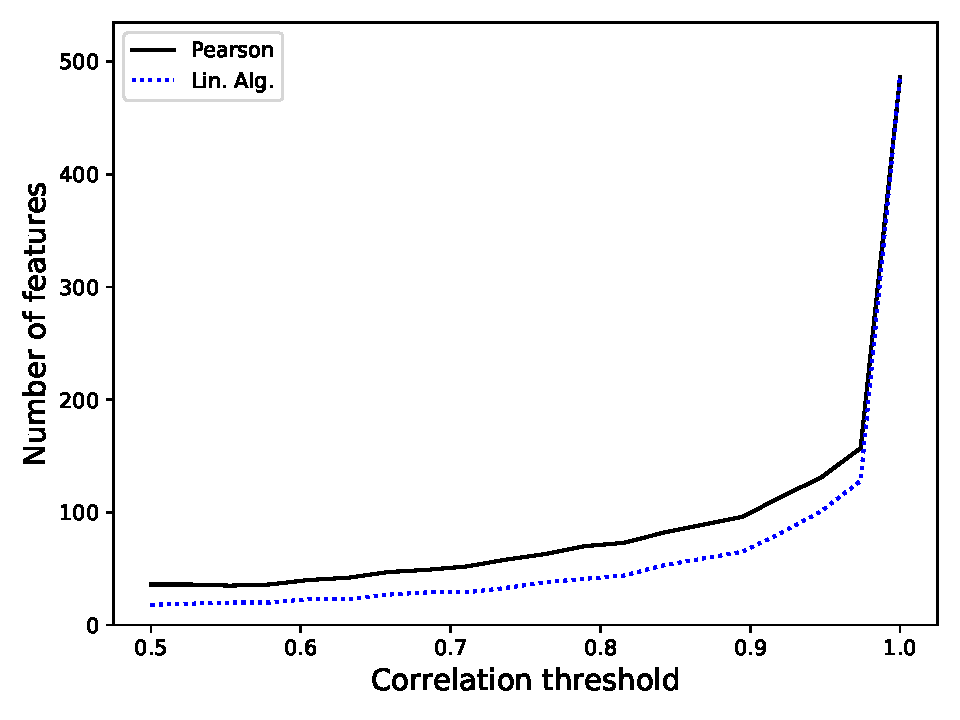
\includegraphics[width=0.8\linewidth]{../output/features/figures/global_max_feature_correlation}
			\end{center}
		\end{column}
	\end{columns}
\end{frame}

%%%%%%%%%%%%%%%%%%%%%%%%%%%%%%%%%%%%%%%%%%%%%%%%%%%%%%%%%%%%%%%%%%%%%%%%%%%%%%%%%%%%%%%%%%%%%%%%%%%%%%%%%%%%%%

\section{Previous Models}
\subsection{}

\begin{frame}[t]\frametitle{Previous Model Performance}
	\begin{minipage}{\linewidth}
		\begin{table}
			\centering
			\begin{tabular}{|c|c|c|c|c|c|}
				\hline
				\multirow{2}{*}{\textbf{Rank}} & \multirow{2}{*}{\textbf{Model}} & \multicolumn{2}{c|}{\textbf{Accuracy}} & \multirow{2}{*}{\textbf{Domain}} & \multirow{2}{*}{\textbf{Normalization}} \\ \cline{3-4}
				& & \textbf{Optimized} & \textbf{HW 3} & & \\ \hline \hline
				1 & \makecell{Perceptron\\Forest} & \makecell{(0.9956,\\1.0000)} & \makecell{(0.9866,\\1.0000)} & Global & Any \\ \hline
				1\footnote{McNemar test \cite{Raschka}.} & KNN & \makecell{(0.9949,\\1.0000)} & \makecell{(0.9814,\\0.9952)} & Global & Standard \\ \hline
				1 & \makecell{Decision\\Tree} & \makecell{(0.9871,\\1.0000)} & \makecell{(0.9914,\\1.0000)} & Global & Any \\ \hline
				1 & Perceptron & \makecell{(0.9871,\\0.9981)} & \makecell{(0.9315,\\0.9600)} & Global & Standard \\ \hline
			\end{tabular}
		\end{table}
	\end{minipage}
	\vspace{-0.3cm}
\end{frame}

\begin{frame}[t]\frametitle{Grid Search}

	\begin{figure}
		\begin{subfigure}{0.45\linewidth}
			\centering
			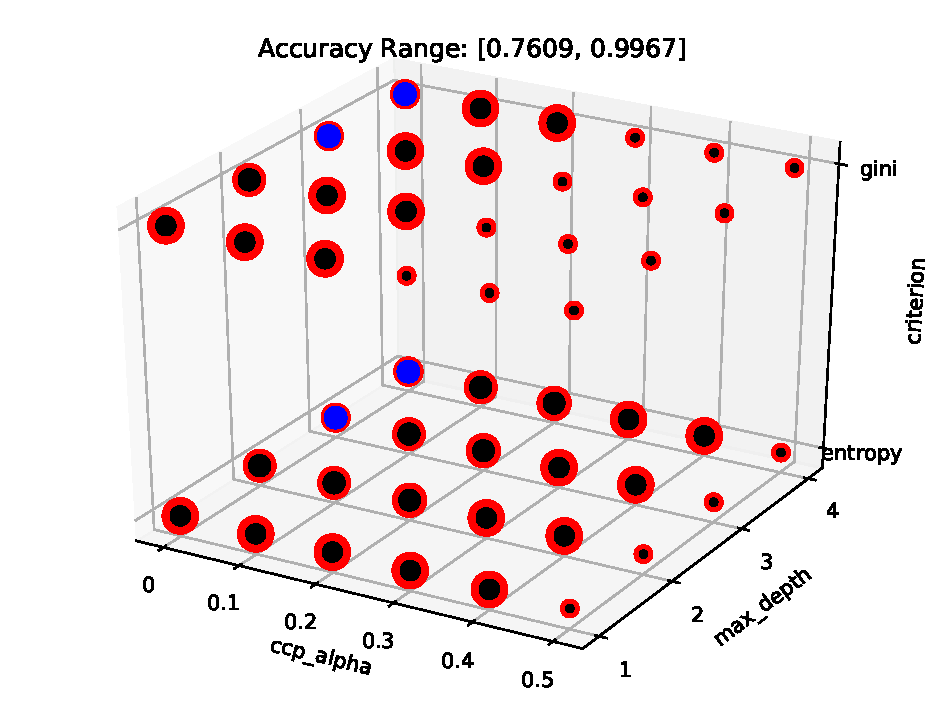
\includegraphics[scale=0.225]{../output/DT/DT_941_486/DT_gridsearch_941_486_global_standard.pdf}
			\caption{Decision tree.}
		\end{subfigure}
		\begin{subfigure}{0.45\linewidth}
			\centering
			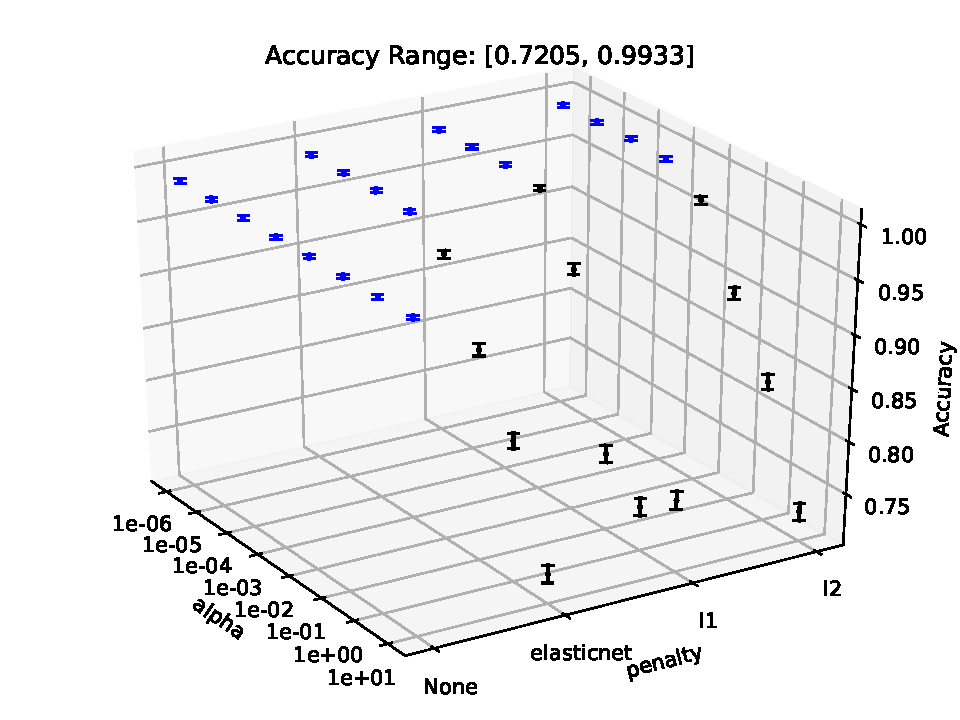
\includegraphics[scale=0.225]{../output/Perceptron/P_941_486/P_gridsearch_941_486_global_standard.pdf}
			\caption{Perceptron.}
		\end{subfigure}
		\begin{subfigure}{0.45\linewidth}
			\centering
			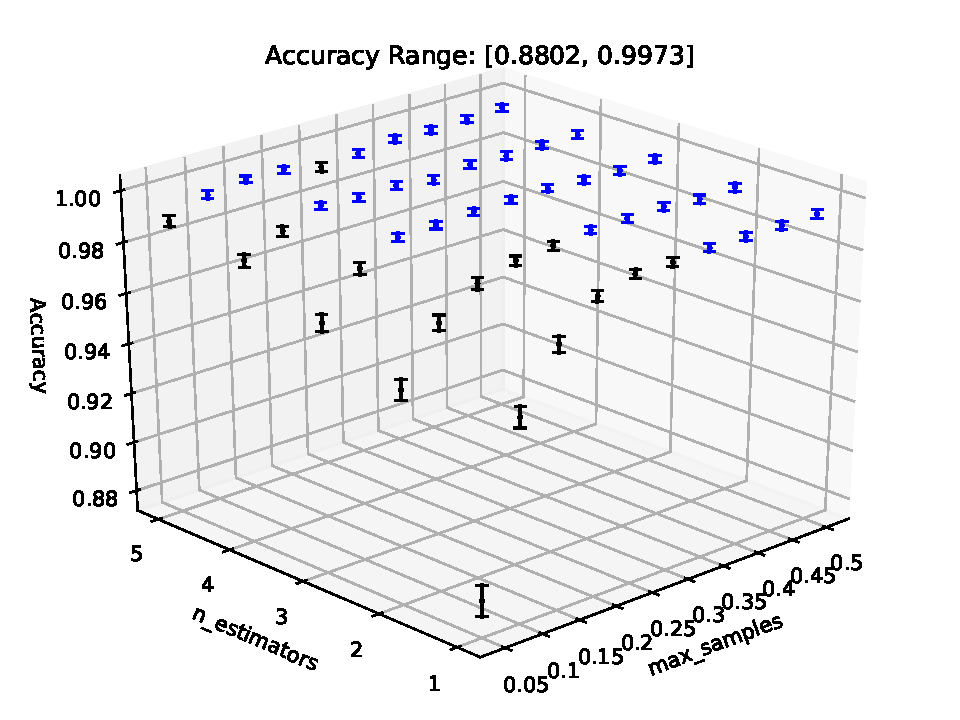
\includegraphics[scale=0.225]{../output/PF/PF_941_486/PF_gridsearch_941_486_global_standard.pdf}
			\caption{Perceptron forest.}
		\end{subfigure}
		\begin{subfigure}{0.45\linewidth}
			\centering
			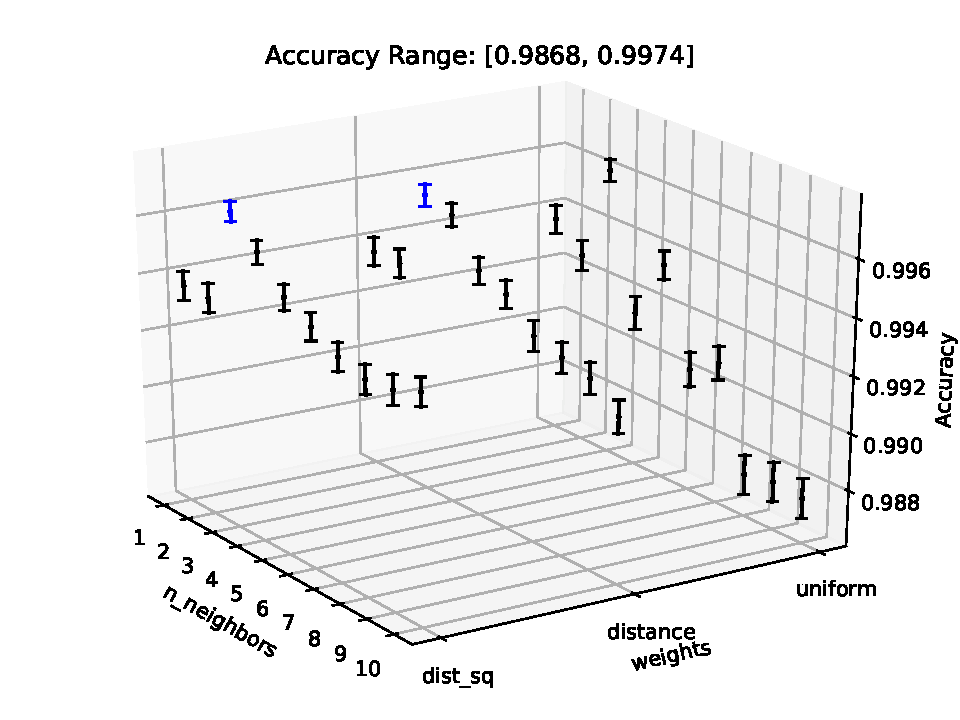
\includegraphics[scale=0.225]{../output/KNN/KNN_941_486/KNN_gridsearch_941_486_global_standard.pdf}
			\caption{KNN.}
		\end{subfigure}
	\end{figure}
\end{frame}

%%%%%%%%%%%%%%%%%%%%%%%%%%%%%%%%%%%%%%%%%%%%%%%%%%%%%%%%%%%%%%%%%%%%%%%%%%%%%%%%%%%%%%%%%%%%%%%%%%%%%%%%%%%%%%
 
\section{Neural Network}
\subsection{}

\begin{frame}[t]\frametitle{Neural Network Optimizations I}
	\begin{itemize}
		\item Batch/Mini-batch/Stochastic:
		\begin{figure}
			\begin{subfigure}{0.45\linewidth}
				\centering
				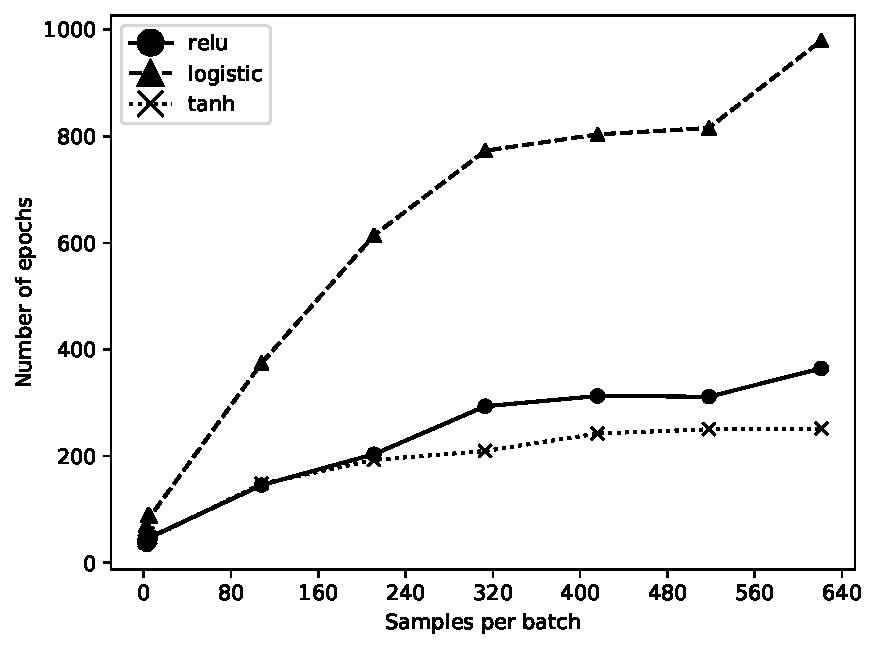
\includegraphics[width=0.9\linewidth]{../output/neural_network/figures/nn_convergence_global_standard_941_486}
			\end{subfigure}
			\begin{subfigure}{0.45\linewidth}
				\centering
				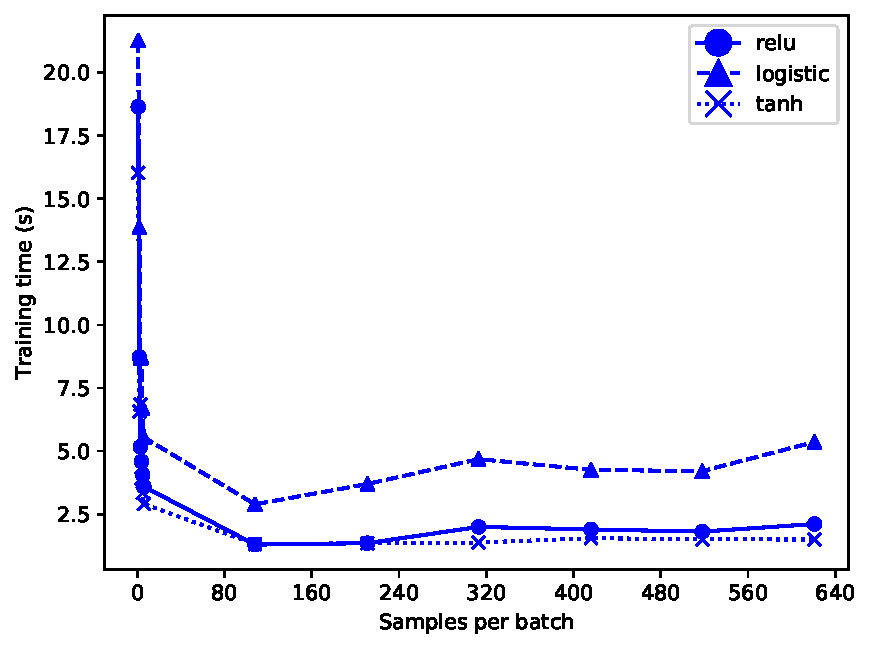
\includegraphics[width=0.9\linewidth]{../output/neural_network/figures/nn_convergence_global_standard_941_486_time}
			\end{subfigure}
		\end{figure}
		\item[-] Number of hidden neurons: 4x7
		\item[-] Stochastic is the best in number of epochs till convergence
		\item[-] Stochastic is the worst in terms of training time (due to large number of parameters)
		\item[-] Both tanh(x) and ReLU(x) activation functions perform better than the sigmoid 
	\end{itemize}
\end{frame}

\begin{frame}[t]\frametitle{Neural Network  Optimizations II}
\begin{itemize}
	\item Number of layers, number of neurons per layer:
	\begin{figure}
		\begin{subfigure}{0.45\linewidth}
			\centering
			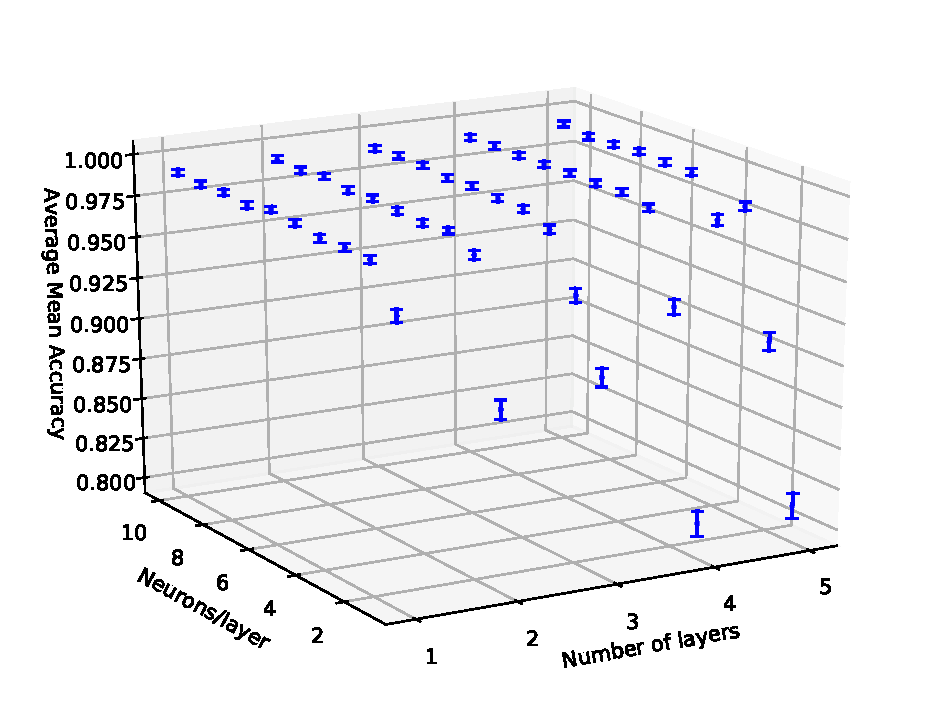
\includegraphics[width=1.0\linewidth]{../output/neural_network/figures/nn_architecture_global_standard_941_486}
			\caption{Number of features: 486}
		\end{subfigure}
		\begin{subfigure}{0.45\linewidth}
			\centering
			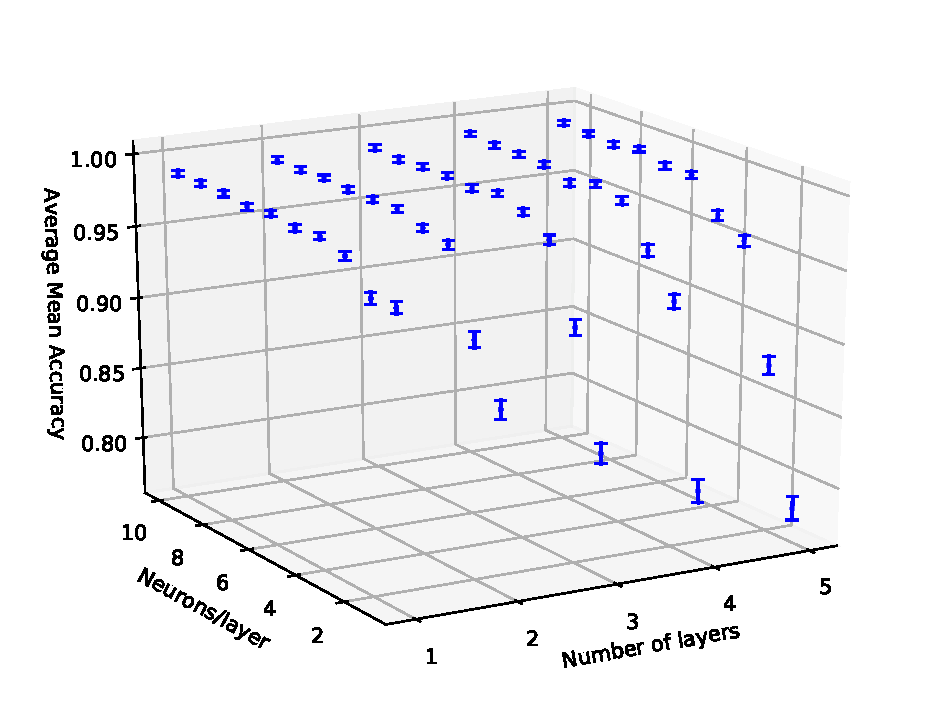
\includegraphics[width=1.0\linewidth]{../output/neural_network/figures/nn_architecture_global_standard_941_486_feature_pearson_90}
			\caption{Number of features: 101}
		\end{subfigure}
	\end{figure}

	\item[-] Connecting multiple layers with only one neuron is not worth it.
	\item[-] Above 6-7 neurons per layer, no statistical improvement observed.
	\item[-] Removing redundant features has little impact on accuracy.
\end{itemize}
\end{frame}
\centering
\begin{frame}[t]\frametitle{Best Neural Network Results}
	\begin{table}[H]
		\small
		\centering
		\begin{tabular}{|c|c|}
			\hline
                         \textbf{Attribute} & \textbf{Value} \\ \hline \hline
			Normalization         &Global Standardization \\ \hline
			Number of layers     & 2 \\ \hline
			Neurons per layer    & 9  \\ \hline
			Mean Accuracy        & 0.9936 \\ \hline
			Standard Deviation   & 0.0026 \\ \hline
			95.00\% Confidence   & 0.9936 $\pm$ 0.0051   \\ \hline
			Accuracy Range       & (0.9885, 0.9987)      \\ \hline
			Best Accuracy        & 0.9968                \\ \hline
			Training Time        & 7.5350 s              \\ \hline
			Classification Time  & 0.0039 s               \\ \hline
		\end{tabular}
	\end{table}
\vskip 0.3cm
Slow to train and not necessarily better than other learners!
\end{frame}

%%%%%%%%%%%%%%%%%%%%%%%%%%%%%%%%%%%%%%%%%%%%%%%%%%%%%%%%%%%%%%%%%%%%%%%%%%%%%%%%%%%%%%%%%%%%%%%%%%%%%%%%%%%%%%

\section{Novel Learner}
\subsection{}

\begin{frame}[t]\frametitle{Ensemble Network Motivation}

\begin{itemize}
	\item Training neural networks is expensive.
	
	\item Employing a bagger as a filter could reduce the dimensionality of the input data and simplify the target function a neural network must learn.
	
	\item Baggers have been shown to be more accurate with unstable weak learners.
	\begin{itemize}
		\item Unstable $\equiv$ Sensitive to training data.
		\item If classifiers within an ensemble have uncorrelated outputs, the output of the ensemble will have higher accuracy than the individual classifiers.
		\item The author's of \cite{ensemble-lit1} show this by comparing unstable decision trees to stable naive Bayes learners.
	\end{itemize}

\item An ensemble approach with decision trees is the appropriate design for the novel learner.
\end{itemize}

\end{frame}


\begin{frame}[t]\frametitle{Ensemble Network Algorithm}
	\begin{center}
		\makebox[\linewidth][c]{	
			\begin{tikzpicture}[scale=0.3]
			% get node at origin
			% variable definitions
			\def\s{3.}; % size of each DT input square
			\def\vertOffset{0.5*\s}; % distance to offset next box above previous
			\def\r{1.5*\s}; % perceptron radius
			\def\d{6*\s}; % distance between inputs and perceptron
			\def\picWidth{3.0};
			
			% draw perceptron
			\draw[fill=cyan] (\d, 0) circle (\r) node {Neural Network};
			
			% draw bias
			\def\i{2}
			\node at (0.5*\s, {\i*(\s + \vertOffset)}) {1};
%			\node[anchor=south] at (0.5*\s, {\i*(\s + \vertOffset) + 0.8*\s}) {Decision tree output = perceptron input};
			\node[anchor=south] at (0.5*\s, {\i*(\s + \vertOffset) + 0.5*\s}) {$x_0$};
			% put box around tree
			\draw (0, {\i*(\s + \vertOffset) - 0.5*\s}) rectangle (\s, {\i*(\s + \vertOffset) + 0.5*\s});
			% draw line from box to perceptron
			\draw (\s, {\i*(\s + \vertOffset)}) -- (\d-\r,0);
			% label line with bias
			\path (\s, {\i*(\s + \vertOffset)}) -- (\d-\r,0) node[midway,above] {$b$};
			
			% draw DTs
			\draw (0.5*\s, 0) circle (0.0) node {\vdots};
			\foreach \i / \ID / \j in {1/1/1, -1/2/N-1, -2/13/N}
			{
				% insert tree
				\node at (0.5*\s, {\i*(\s + \vertOffset)}) {\includegraphics[width=1cm]{../output/PF/PF_941_486/PF_DT\ID_best.gv.pdf}};
				\node[anchor=south] at (0.5*\s, {\i*(\s + \vertOffset) + 0.5*\s}) {$x_{\j}$};
				% put box around tree
				\draw (0, {\i*(\s + \vertOffset) - 0.5*\s}) rectangle (\s, {\i*(\s + \vertOffset) + 0.5*\s});
				% draw line from box to perceptron
				\draw (\s, {\i*(\s + \vertOffset)}) -- (\d-\r,0);
				% label line with weight
				\path (\s, {\i*(\s + \vertOffset)}) -- (\d-\r,0) node[midway,above] {$w_{\j}$};
			}
			\end{tikzpicture}
		}
	\end{center}
\end{frame}

\begin{frame}[t]\frametitle{Ensemble Network Architecture Optimization}
	\begin{itemize}
		\item Number of estimators, network architecture:
		\begin{figure}
			\begin{subfigure}{0.45\linewidth}
				\centering
				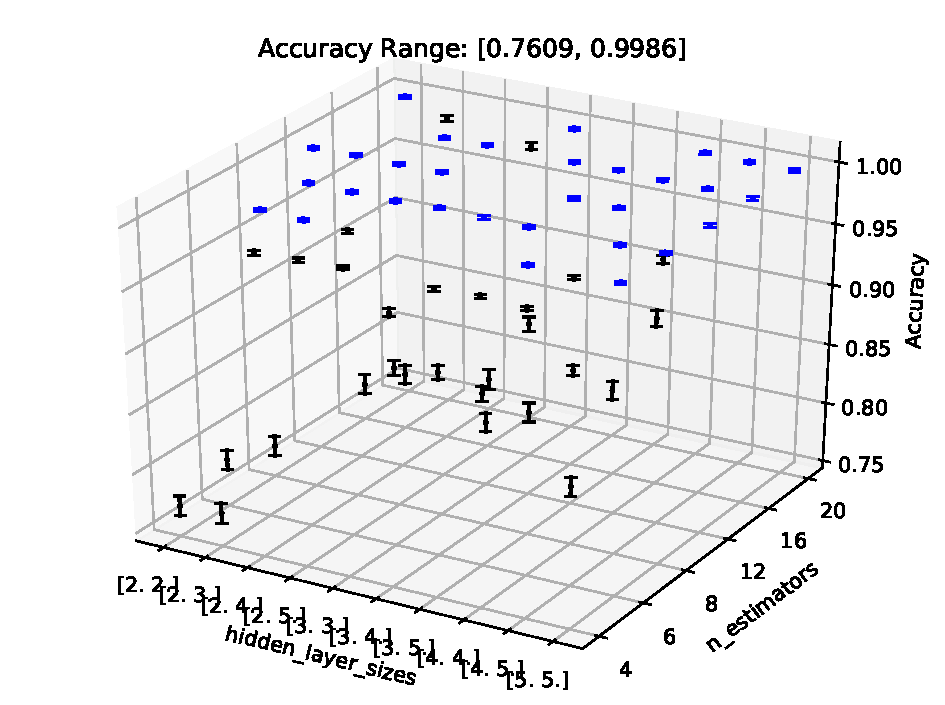
\includegraphics[width=1.0\linewidth]{../output/EN/EN_941_486/EN_gridsearch_941_486_global_max_range26.pdf}
			\end{subfigure}
			\begin{subfigure}{0.45\linewidth}
				\centering
				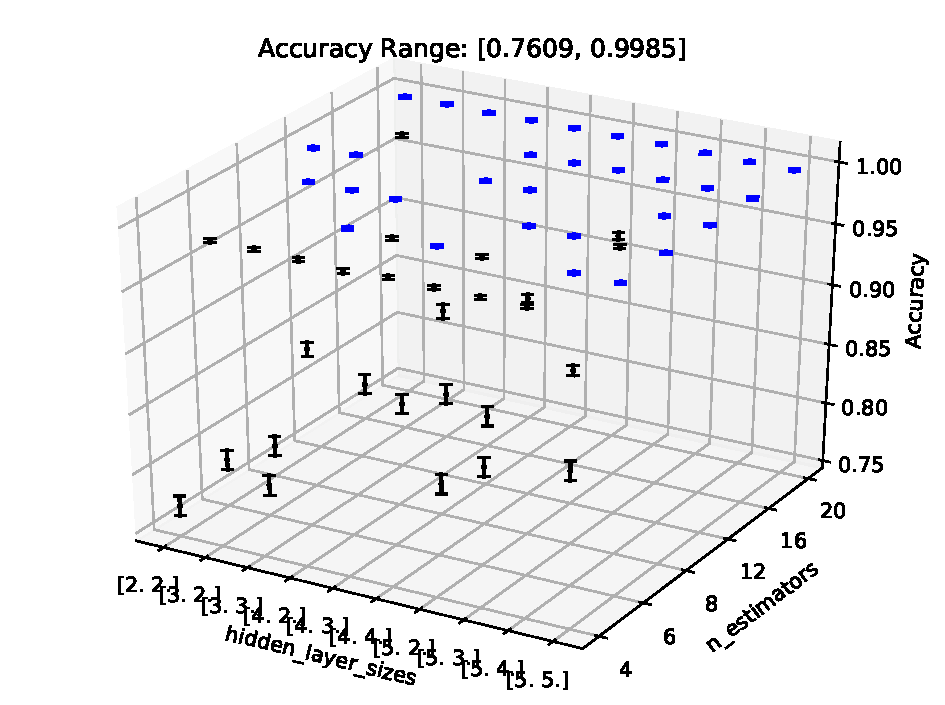
\includegraphics[width=1.0\linewidth]{../output/EN/EN_941_486/EN_gridsearch_941_486_global_max_range51.pdf}
			\end{subfigure}
		\end{figure}
		
		\item[-] Significant reduction in overall size of neural network.
		\item[-] Optimum number of hidden layers 2.
		\item[-] Best Configuration:
		\begin{itemize}
			\item[*] Number of estimators: 8
			\item[*] Architecture: (3, 3)
		\end{itemize}
	\end{itemize}
\end{frame}

\begin{frame}[t]\frametitle{Best Ensemble Network Results}
	\begin{table}[H]
		\small
		\centering
		\begin{tabular}{|c|c|}
			\hline
			\textbf{Attribute} & \textbf{Value} \\ \hline \hline
			Normalization	& Global Standardization \\ \hline
			Mean Accuracy        & 0.9979 \\ \hline
			Standard Deviation   & 0.0015 \\ \hline
			95.00\% Confidence   & 0.9979 $\pm$ 0.0048 \\ \hline
			Accuracy Range       & (0.9931, 1.0000) \\ \hline
			Best Accuracy        & 1.0000 \\ \hline
			Training Time        & 2.5403 s\\ \hline
			Classification Time  & 0.0242 s \\ \hline
		\end{tabular}
	\end{table}
	\begin{center}
		Greatest mean accuracy of all models and $\approx 66\%$ reduction in training time compared to the neural network!
	\end{center}
	\vskip 0.5cm
\end{frame}

%%%%%%%%%%%%%%%%%%%%%%%%%%%%%%%%%%%%%%%%%%%%%%%%%%%%%%%%%%%%%%%%%%%%%%%%%%%%%%%%%%%%%%%%%%%%%%%%%%%%%%%%%%%%%%

\section{Performance Comparisons}
\subsection{}

\begin{frame}[t]\frametitle{Model Comparisons}
\begin{minipage}{\linewidth}
	\begin{table}
		\centering
		\begin{tabular}{|c|c|c|c|c|c|}
			\hline
			\multirow{2}{*}{\textbf{Rank}} & \multirow{2}{*}{\textbf{Model}} & \multicolumn{2}{c|}{\textbf{Accuracy}} & \multirow{2}{*}{\textbf{Domain}} & \multirow{2}{*}{\textbf{Normalization}} \\ \cline{3-4}
			& & \textbf{Optimized} & \textbf{HW 3} & & \\ \hline \hline
			1 & \makecell{Perceptron\\Forest} & \makecell{(0.9956,\\1.0000)} & \makecell{(0.9866,\\1.0000)} & Global & Any \\ \hline
			1 & KNN & \makecell{(0.9949,\\1.0000)} & \makecell{(0.9814,\\0.9952)} & Global & Standard \\ \hline
			\textcolor{blue}{1} & \textcolor{blue}{\makecell{Ensemble\\Network}} & \textcolor{blue}{\makecell{(0.9931,\\1.0000)}} & \textcolor{blue}{--} & \textcolor{blue}{Global} & \textcolor{blue}{Any} \\ \hline
			\textcolor{blue}{1} & \textcolor{blue}{\makecell{Neural\\Network}} & \textcolor{blue}{\makecell{(0.9885,\\0.9987)}} & \textcolor{blue}{--} & \textcolor{blue}{Global} & \textcolor{blue}{Standard} \\ \hline
			1 & \makecell{Decision\\Tree} & \makecell{(0.9871,\\1.0000)} & \makecell{(0.9914,\\1.0000)} & Global & Any \\ \hline
			1 & Perceptron & \makecell{(0.9871,\\0.9981)} & \makecell{(0.9315,\\0.9600)} & Global & Standard \\ \hline
		\end{tabular}
	\end{table}
\end{minipage}
\vspace{-0.3cm}
\end{frame}

%%%%%%%%%%%%%%%%%%%%%%%%%%%%%%%%%%%%%%%%%%%%%%%%%%%%%%%%%%%%%%%%%%%%%%%%%%%%%%%%%%%%%%%%%%%%%%%%%%%%%%%%%%%%%%

\section{Conclusion}
\subsection{}

\begin{frame}[t]\frametitle{Conclusions}
	\begin{itemize}
		\item For neural networks, $\tanh(x)$ and mini-batch learning yield the minimum training times.
		\vspace*{0.1in}
		
		\item The novel learner yielded comparable to better accuracy to the neural network. \vspace*{0.1in}
	
		\item The novel learner sports a 66\% reduction in training time compared to the neural network.
		\vspace*{0.1in}
		
		\item Further optimizations on the novel learner architecture and exploration of PCA to come!
		
	\end{itemize}
\end{frame}

\begin{frame}[t]\frametitle{References}
	\bibliographystyle{ieeetr}
	%custom ANS journal submission template bibliography style
	\bibliography{bibliography}
\end{frame}

\end{document}
